\myPara{Text Alignment}
% \dq{@Tianqi, Weijie, Daquan}
One of the key metrics for video generative models is their ability to follow text prompts accurately. This capability is essential for the effectiveness of these models. However, some open-source models often struggle to capture all subjects or accurately represent the relationships between multiple subjects, particularly when the input text prompt is complex.
%
\nameofmethod{} demonstrates robust capabilities in generating videos that closely adhere to the provided text prompts. As illustrated in Figure \ref{fig:text-align}, it effectively manages multiple subjects within the scene.

\begin{figure}[h]
    \centering
    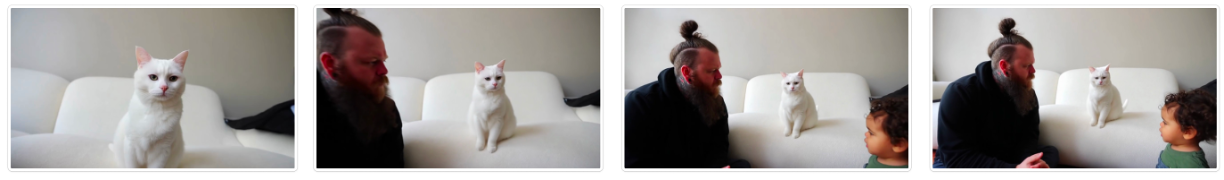
\includegraphics[width=\linewidth]{figures/text_alignment.png}
    \caption{{Prompt: A white cat sits on a white soft sofa like a person, while its long-haired male owner, with his hair tied up in a topknot, sits on the floor, gazing into the cat's eyes. His child stands nearby, observing the interaction between the cat and the man. } }
    \label{fig:text-align}
\end{figure}